\clearpage
\setcounter{page}{1}
\maketitlesupplementary



\section{Methods Supplementary}
\subsection{Aggregation role of ReID loss functions}
Currently, ReID models commonly use cross-entropy loss to impose ID-level constraints, and contrastive losses (such as triplet loss) to bring features of the same ID closer while pushing apart features of different IDs. Some models also utilize center loss to construct identity centers for dynamically constraining the IDs. These methods lead to one common result: feature aggregation. From the perspective of the gradient of the loss functions, we could prove that the feature vectors of each ID in current ReID tasks naturally aggregate around a center or mean in the followings.
\paragraph{Cross-Entropy Loss} 
is often used in classification tasks, optimizing the model by maximizing the probability of the correct class. Given $N$ samples, each with a feature vector $\mathbf{z}_i \in \mathbb{R}^d$, and its corresponding class label $y_i \in \{1, 2, \dots, C\}$, the cross-entropy loss is defined as:
\begin{equation}
\mathcal{L}_{\text{CE}} = -\frac{1}{N} \sum_{i=1}^{N} \log \frac{\exp(\mathbf{w}_{y_i}^\top \mathbf{z}_i + b_{y_i})}{\sum_{j=1}^{C} \exp(\mathbf{w}_j^\top \mathbf{z}_i + b_j)}
\end{equation}
where $\mathbf{w}_j$ and $b_j$ are the weight vector and bias for class $j$, respectively.

For simplicity, assume that the final layer is a linear classifier without bias, i.e., $b_j = 0$. When the loss is minimized, the optimization objective is to maximize the score $\mathbf{w}_{y_i}^\top \mathbf{z}_i$ of the correct class while minimizing the scores $\mathbf{w}_j^\top \mathbf{z}_i$ of other classes ($j \neq y_i$).

By gradient descent optimization, we can obtain:
\begin{equation}
\frac{\partial \mathcal{L}_{\text{CE}}}{\partial \mathbf{z}_i} = 1/N\left(p_{y_i} - 1\right) \mathbf{w}_{y_i} + 1/N\sum_{j \neq y_i} p_{ij} \mathbf{w}_j
\end{equation}
where $p_{ij} = \frac{\exp(\mathbf{w}_j^\top \mathbf{z}_i)}{\sum_{k=1}^{C} \exp(\mathbf{w}_k^\top \mathbf{z}_i)}$.

With the loss function converges, $p_{y_i}\rightarrow1$ and $p_{ij}\rightarrow0 (j \neq y_i)$. The feature $\mathbf{z}_i$ is optimized to be near a linear combination of the class weight vectors $\mathbf{w}_{y_i}$. This indicates that features of the same class will tend toward a common direction, thus achieving feature aggregation.

\paragraph{Contrastive loss} (Triplet Loss as example) optimizes the feature space by bringing samples of the same class closer and pushing samples of different classes further apart. A triplet $(\mathbf{z}_a, \mathbf{z}_p, \mathbf{z}_n)$ is defined, where $\mathbf{z}_a$ is the anchor, $\mathbf{z}_p$ is the positive sample (same class), and $\mathbf{z}_n$ is the negative sample (different class). The triplet loss is defined as:
\begin{equation}
\mathcal{L}_{\text{Triplet}} = \max \left( \| \mathbf{z}_a - \mathbf{z}_p \|_2^2 - \| \mathbf{z}_a - \mathbf{z}_n \|_2^2 + \alpha, 0 \right)
\end{equation}
where $\alpha$ is the margin parameter.

To minimize the loss, the optimization objective is:
\begin{equation}
\| \mathbf{z}_a - \mathbf{z}_p \|_2^2 + \alpha < \| \mathbf{z}_a - \mathbf{z}_n \|_2^2
\end{equation}
\begin{align}
\frac{\partial \mathcal{L}_{\text{Triplet}}}{\partial \mathbf{z}_a} &= 2 (\mathbf{z}_n - \mathbf{z}_p), \\
\frac{\partial \mathcal{L}_{\text{Triplet}}}{\partial \mathbf{z}_p} &= 2 (\mathbf{z}_p - \mathbf{z}_a), \\
\frac{\partial \mathcal{L}_{\text{Triplet}}}{\partial \mathbf{z}_n} &= 2 (\mathbf{z}_a - \mathbf{z}_n).
\end{align}

By minimizing triplet loss, the feature $\mathbf{z}_p$ is pulled closer to $\mathbf{z}_a$, while $\mathbf{z}_n$ is pushed away. Through this mechanism, Triplet Loss encourages features of the same class to aggregate together while features of different classes are separated from each other.

\paragraph{Center loss} further enhances feature aggregation by introducing a feature center for each class. For each class $j$, there is a feature center $\mathbf{c}_j$, and the center loss is defined as:
\begin{equation}
\mathcal{L}_{\text{Center}} = \frac{1}{2} \sum_{i=1}^{N} \| \mathbf{z}_i - \mathbf{c}_{y_i} \|_2^2
\end{equation}

The goal of minimizing center loss is to make each sample's feature vector $\mathbf{z}_i$ as close as possible to its corresponding class center $\mathbf{c}_{y_i}$. Through gradient descent, we obtain:
\begin{align}
\frac{\partial \mathcal{L}_{\text{Center}}}{\partial \mathbf{z}_i} &= \mathbf{z}_i - \mathbf{c}_{y_i} \\
\frac{\partial \mathcal{L}_{\text{Center}}}{\partial \mathbf{c}_j} &= \begin{cases}
\mathbf{c}_j - \mathbf{z}_i & \text{if } y_i = j \\
0 & \text{otherwise}
\end{cases}
\end{align}

Thus, the optimization process not only pulls sample features closer to their centers but also dynamically updates each class's center to represent the mean of that class's feature distribution. This directly encourages features of the same class to aggregate together.



% \paragraph{Limb Length Constraints}

% Let \( \mathbf{k}_i = (x_i, y_i) \) represent the normalized coordinates of the \( i \)-th keypoint in the image. The Euclidean distance between two keypoints \( \mathbf{k}_i \) and \( \mathbf{k}_j \), corresponding to body joints, is given by:
% \begin{equation}
% d(\mathbf{k}_i, \mathbf{k}_j) = \sqrt{(x_i - x_j)^2 + (y_i - y_j)^2}
% \end{equation}

% For example, the length of the left arm, denoted as \( d_{\text{left arm}} \), is calculated as the distance between the left shoulder and left elbow keypoints:
% \begin{equation}
% d_{\text{left arm}} = d(\mathbf{k}_{\text{LS}}, \mathbf{k}_{\text{LE}})
% \end{equation}
% \begin{equation}
% d_{\text{right arm}} = d(\mathbf{k}_{\text{RS}}, \mathbf{k}_{\text{RE}})
% \end{equation}

% We ensure that limb lengths fall within a reasonable range, defined by the minimum and maximum allowable limb lengths:
% \begin{equation}
% l_{\text{min}} \leq d_{\text{left arm}}, d_{\text{right arm}}, d_{\text{left leg}}, d_{\text{right leg}} \leq l_{\text{max}}
% \end{equation}


% \paragraph{Positional Constraints}

% Finally, we apply positional constraints to ensure keypoints are in anatomically plausible positions. For example, the head \( \mathbf{k}_{\text{H}} \) must be higher than the center of the body \( \mathbf{k}_{\text{C}} \) and the knees must be positioned below the hips:
% \begin{equation}
% y_{\text{H}} < y_{\text{C}}
% \end{equation}
% \begin{equation}
% y_{\text{LK}} > y_{\text{LH}}, \quad y_{\text{RK}} > y_{\text{RH}}
% \end{equation}

% \subsubsection{Identity Feature Redistribution}

% We use the pretrained ReID model to extract identity features:
% \begin{equation}
% \mathbf{f} = \text{ReID}(\mathbf{x}^{\text{ref}})
% \end{equation}

% On this basis, we design a learnable Feature Re-Distribution mapping module (IFR) to allow the model to optimize the feature distribution $\mathbf{f} \in \mathbb{R}^d$ while reducing the interference of feature noise on the diffusion model. Then use this as the conditioning embedding \( \mathbf{H} \in \mathbb{R}^{N \times D} \):
% \begin{equation}
% \mathbf{H} = \text{IFR}(\mathbf{f})
% \end{equation}

% The ReID Prompt Module projects and concatenates the features:
% \begin{align}
% \mathbf{h} &= \text{Linear}_{\text{ReID}}(\mathbf{f}) \in \mathbb{R}^{N \times D} \\
% \mathbf{H} &= \text{LayerNorm}(\mathbf{h})
% \end{align}
% where \( N \) is the sequence length, and \( D \) is the feature dimension.




\subsection{Identity Density ($\text{ID}^2$) Metric}
Identity density is one aspect of measuring ReID effectiveness. However, there is currently no quantitative metric for this, and researchers commonly rely on visualization tools like t-SNE to demonstrate model performance. Due to the large number of IDs, this approach is limited to visualizing only a few IDs, making it challenging to assess model performance from a global perspective quantitatively. Some researchers exploit this limitation by selecting the best-performing IDs of their models for visualization. To address this, we propose an Identity Density ($\text{ID}^2$) Metric. This metric evaluates the global ID aggregation performance by taking each ID center across the entire test set (gallery and query) as a benchmark.
\begin{equation}
\text{ID}^2 = \frac{1}{N} \sum_{i=1}^{N} \frac{1}{n_i} \sum_{j=1}^{n_i} d\left( \frac{f_{ij}}{\|f_{ij}\|_2}, c_i \right)
\end{equation}
where \( N \) is the total number of unique IDs in the test set, and \( n_i \) is the number of samples for ID \( i \). The feature vector of the \( j \)-th sample of ID \( i \) is denoted as \( f_{ij} \), and \( c_i \) represents the identity center of ID \( i \), computed as follows:
\begin{equation}
c_i = \frac{1}{n_i} \sum_{j=1}^{n_i} \frac{f_{ij}}{\|f_{ij}\|_2}
\end{equation}

Both the feature vectors \( f_{ij} \) and the identity centers \( c_i \) are \( L_2 \)-normalized to ensure consistent feature scaling. The function \( d(\cdot, \cdot) \) represents the Euclidean distance. 


\subsection{Pose Encoder Details}

The Pose Encoder module is designed to extract high-dimensional pose embeddings from the input poses. 
\begin{equation}
\mathbf{E}_{\text{pose}} = \text{PoseEncoder}(\mathbf{x}^{\text{pose}})
\end{equation}

The input is a feature map of size \(C_{\text{in}} \times H \times W\), denoted as \( \mathbf{x}^{\text{pose}} \), 
where \(C_{\text{in}}\) is the number of input channels, and \(H, W\) are the height, and width of the input. 
The first convolution layer is defined as:
\begin{equation}
\mathbf{E}_0 = \text{SiLU}(\text{Conv}_{\text{in}}(\mathbf{x}^{\text{pose}}))
\end{equation}
where \( \text{Conv}_{\text{in}} \) is a convolution operation with kernel size \(3 \times 3\), 
and the number of channels changes from \( C_{\text{in}} =3\) to \( C_0 =16\):

Each block applies a normal \(3 \times 3\) Conv, a \(3 \times 3\) Conv with stride 2 to reduce spatial dimensions, and followed by a SiLU activate function.
For the \(i\)-th convolutional block, the operations can be expressed as:
\begin{equation}
\mathbf{E}_{i+1} = \text{SiLU}(\text{Conv}_{i, \text{stride}=2}(\text{Conv}_{i}(\mathbf{E}_i)))
\end{equation}

The number of channels for each block is as follows: $[C_0, C_1, C_2, C_3] = [16, 32, 64, 128]$

The output Conv layer maps the features from the last block to the target embedding dimension \(C_{\text{out}} = 320\), 
expressed as:
\begin{equation}
\mathbf{E}_{\text{pose}} = \text{Conv}_{\text{out}}(\mathbf{E}_4)
\end{equation}


\subsection{Detailed Description of Neighbor Feature Centralization (NFC)}

\paragraph{Step 1: Compute Distance Matrix}

Given all feature vectors in the gallery \(\{\mathbf{z}_i\}_{i=1}^N\), our goal is to enhance each feature vector by aggregating features from its mutual nearest neighbors.
Compute the pairwise distance matrix \(\mathbf{D} = [d_{ij}]\) where \(d_{ij}\) represents the distance between features \(\mathbf{z}_i\) and \(\mathbf{z}_j\). To avoid self-matching, set the diagonal elements to a large constant, i.e. \[d_{ii} = C, \quad \text{for } i = 1, 2, \dots, N\]

\paragraph{Step 2: Find Top \(k_1\) Nearest Neighbors}

For each feature \(\mathbf{z}_i\), find its top \(k_1\) nearest neighbors based on the distance matrix \(\mathbf{D}\). Denote the set of indices of these neighbors as:
\begin{equation}
\mathcal{N}_{i} = \operatorname{TopK}_{k_1}(\{d_{ij}\}_{j=1}^N)
\end{equation}

\paragraph{Step 3: Identify Mutual Nearest Neighbors}

For each feature \(\mathbf{z}_i\), identifies its mutual nearest neighbors by checking whether each neighbor in \(\mathcal{N}_{i}\) also considers \(\mathbf{z}_i\) as one of its top \(k_2\) nearest neighbors. Specifically, for each \(j \in \mathcal{N}_{i}\), checks if \(i \in \mathcal{N}_{j}^{k_2}\), where \(\mathcal{N}_{j}^{k_2}\) is the set of indices of the top \(k_2\) nearest neighbors of \(\mathbf{z}_j\). If this condition is satisfied, add \(j\) to the mutual nearest neighbor set \(\mathcal{M}_{i}\):
\begin{equation}
\mathcal{M}_{i} = \{ j \mid j \in \mathcal{N}_{i}, \, i \in \mathcal{N}_{j}^{k_2} \}
\end{equation}

\paragraph{Step 4: Feature Centralization Enhancement}

Then it could centralize each feature vector \(\mathbf{z}_i\) by aggregating the features of its mutual nearest neighbors:
\begin{equation}
\mathbf{z}_i^{\text{centralized}} = \mathbf{z}_i + \sum_{j \in \mathcal{M}_{i}} \mathbf{z}_j
\end{equation}

This aggregation reduces feature noise and improves discriminability by incorporating information from similar features.

\begin{figure}
\centering
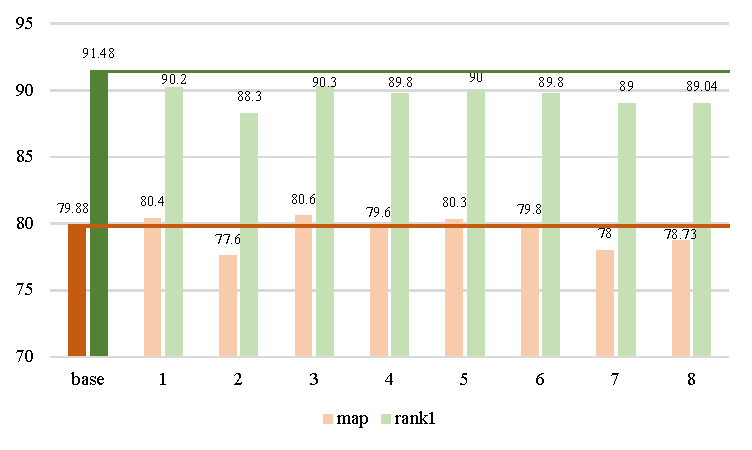
\includegraphics[width=\linewidth]{figs/pdf/samepose.pdf}
\caption{ReID results with images generated with the same pose on Market1501.}
\label{fig:samepose}
\end{figure}

\begin{figure}
\centering
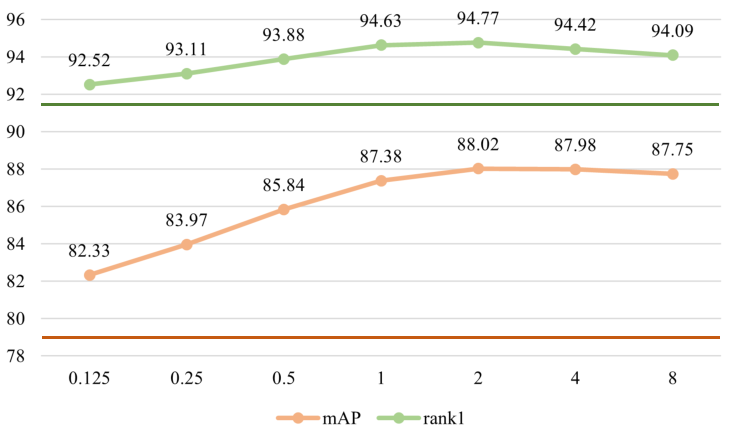
\includegraphics[width=0.9\linewidth]{figs/pdf/eta.pdf}
\caption{Impact of the quality coefficient \( \eta \) with TransReID on Market1501. The dark color lines are the baseline.}
\label{fig:eta}
\end{figure}

\begin{figure}
\centering
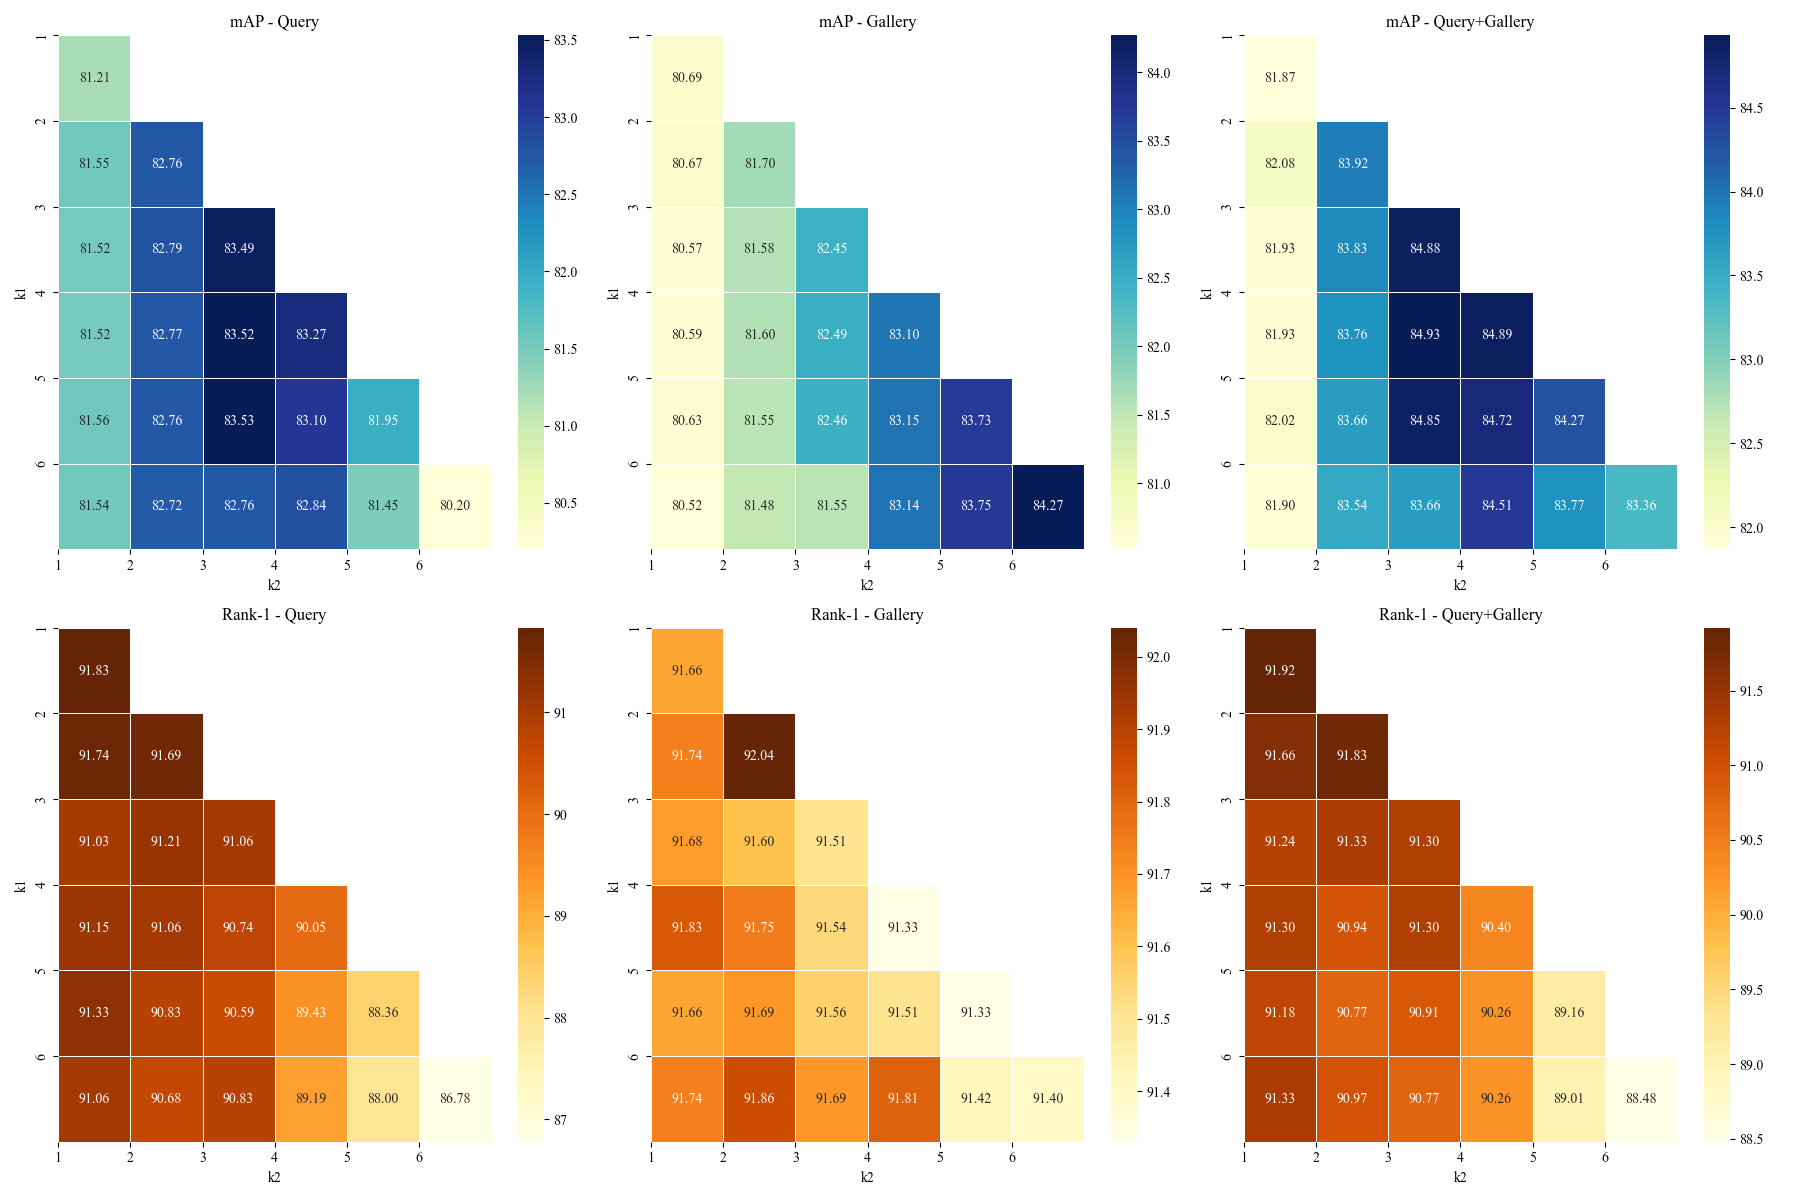
\includegraphics[width=0.9\linewidth]{figs/k1k2.png}
\caption{$k_1/k_2$ analysis of Neighbor Feature Centralization (NFC) with TransReID on Market1501 without re-ranking.}
\label{fig:k1k2}
\end{figure}

\section{Experiments Supplementary}
\begin{figure*}
\centering
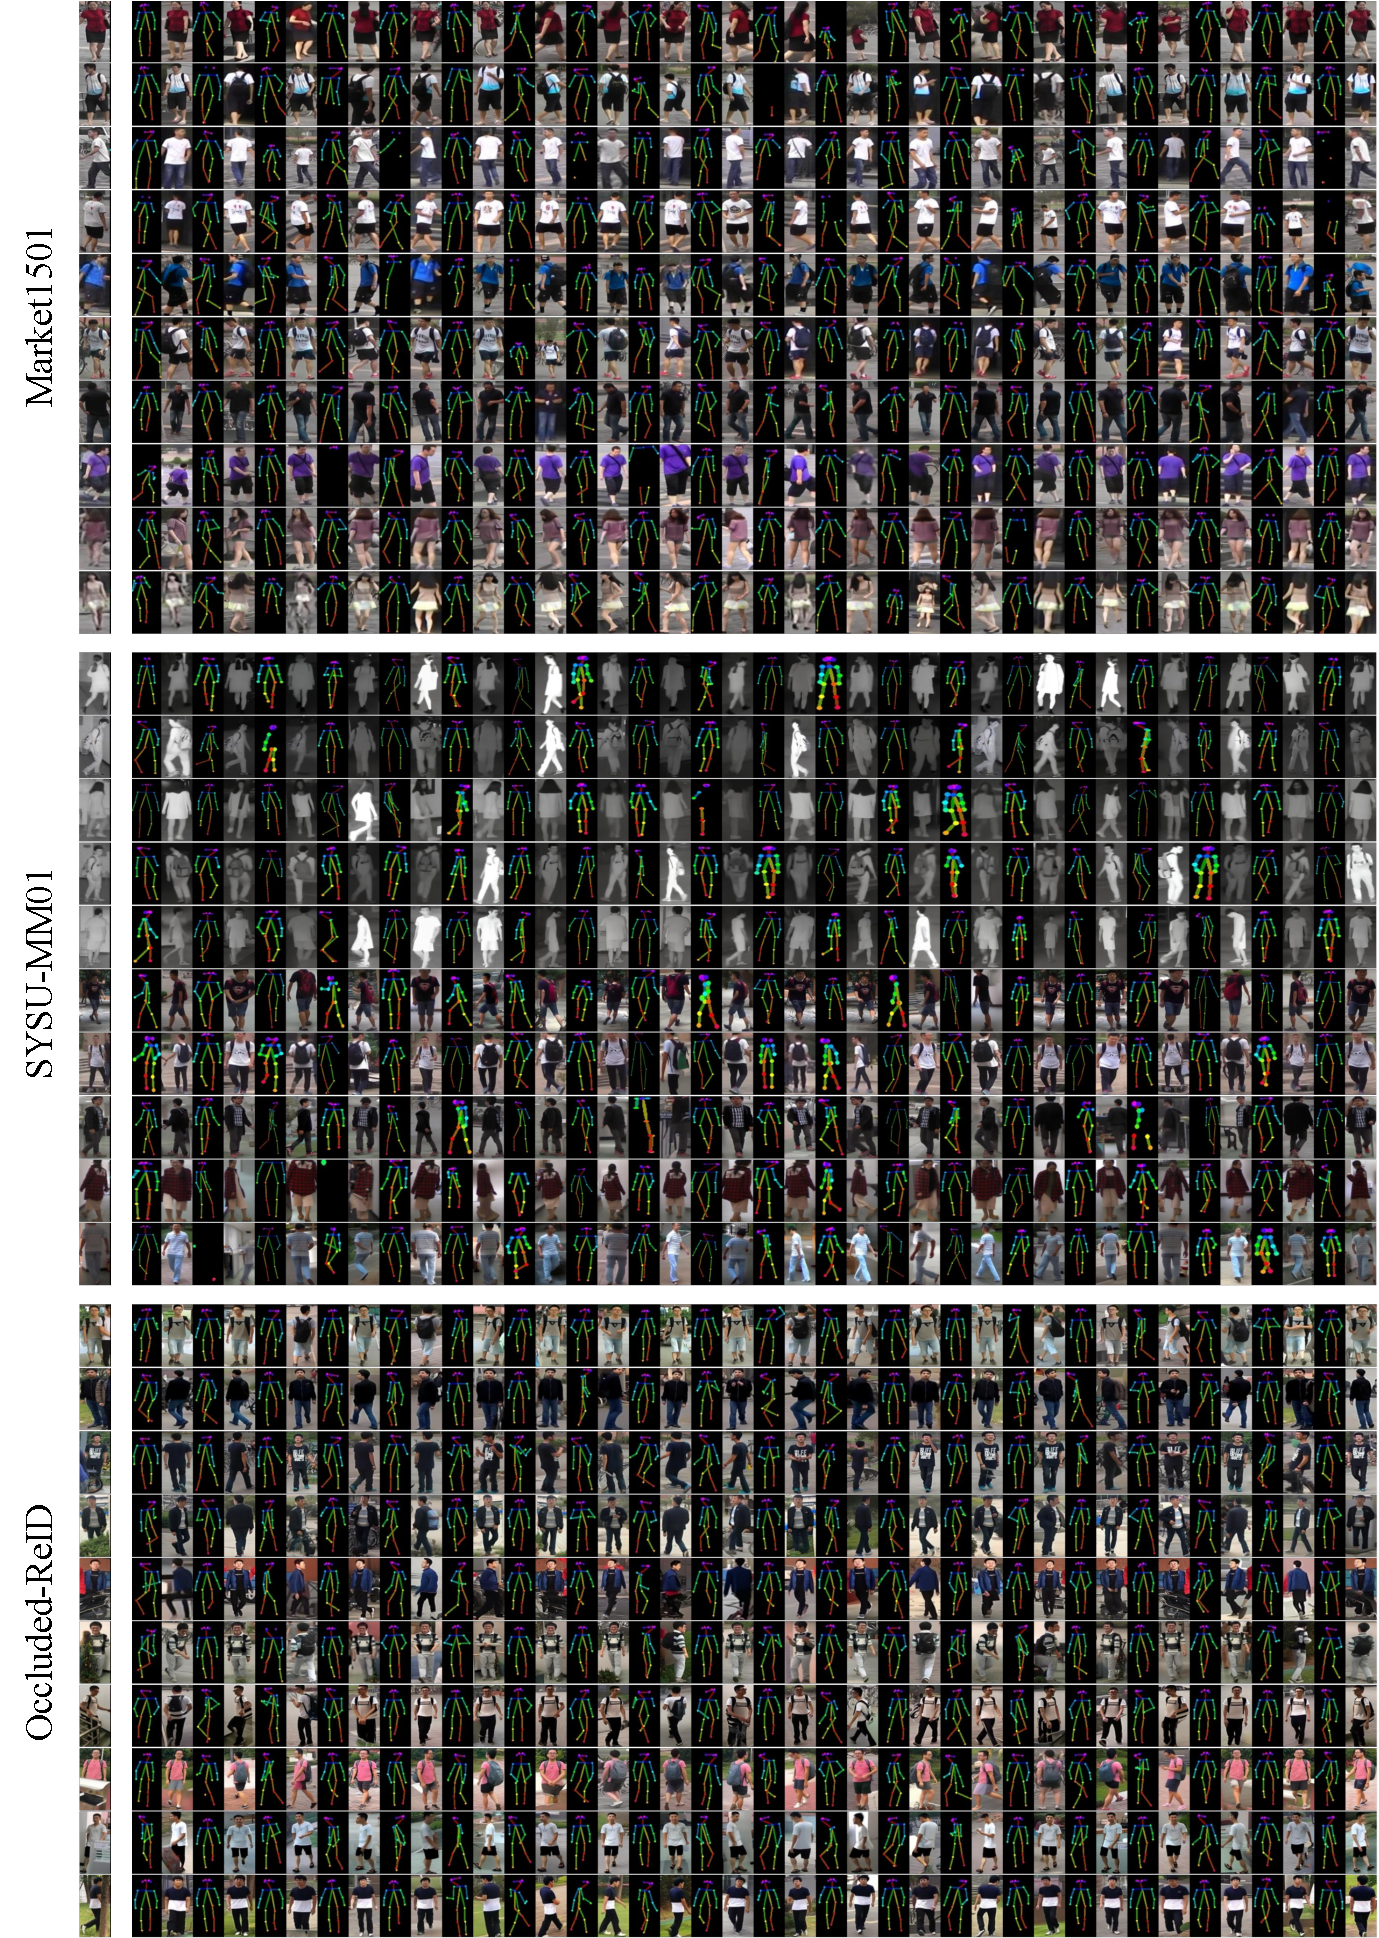
\includegraphics[width=\linewidth]{figs/pdf/random_l.pdf}
\caption{More random generated images on three datasets.}
\label{fig:random_all}
\end{figure*}
\subsection{Data Cleansing}
Training an effective generative model requires high-quality data support. In current ReID (Person Re-Identification) datasets, there are many low-quality images, and removing them can help reduce interference to the model. In our experiments, we found two main issues that need to be addressed: \textbf{Extremely Low-quality Images}: The dataset contains images with such low resolution that even the human eye cannot recognize them as a "person". \textbf{Pose Estimation Failures}: The pose estimation model inevitably fails to detect pedestrian poses in some images.

\subsubsection{Extremely Low-quality Images}

To address this, manual filtering is impractical. Therefore, we designed an automated filtering algorithm. We leverage normal distribution of feature vector, if the feature on the edge of the distribution, largely due to the data itself is out of the distribution of its identity, and it can be picked up. 
% We calculate the mean and covariance matrix of the feature vectors for each ID and filter out samples whose feature distances lie outside a predefined quantile range.

Let \( \mathbf{f}_i \in \mathbb{R}^d \) denote the feature vector of the \( i \)-th sample of a particular identity, where \( d \) is the feature dimension. The mean vector \( \boldsymbol{\mu} \) and covariance matrix \( \boldsymbol{\Sigma} \) are computed as follows:
\begin{equation} 
\boldsymbol{\mu} = \frac{1}{N} \sum_{i=1}^{N} \mathbf{f}_i, \quad \boldsymbol{\Sigma} = \frac{1}{N} \sum_{i=1}^{N} (\mathbf{f}_i - \boldsymbol{\mu})(\mathbf{f}_i - \boldsymbol{\mu})^\top
\end{equation}
where \( N \) is the number of samples for a given ID.

To detect outliers, we compute the Mahalanobis distance \( d_i \) of each feature vector \( \mathbf{f}_i \) from the mean vector \( \boldsymbol{\mu} \), defined as:
\begin{equation}
dis_i = \sqrt{ (\mathbf{f}_i - \boldsymbol{\mu})^\top \boldsymbol{\Sigma}^{-1} (\mathbf{f}_i - \boldsymbol{\mu}) }
\end{equation}

Given that the feature vectors are assumed to follow a multivariate normal distribution, we use quantiles of the Mahalanobis distance to filter out outliers. Specifically, we define a lower bound \( Q_p \) and an upper bound \( Q_{1-p} \) based on the \( p \)-th and \( (1 - p) \)-th quantiles, respectively. Samples with distances outside this range are considered outliers and are removed, and can get a set $S^{\text{ref}}_{i}$ for $i^{th}$ ID:
\begin{equation} \label{outliers}
S_i^{\text{ref}} = \{ \mathbf{x}_i \mid dis_i \in [Q_p, Q_{1-p}] \}
\end{equation}



\begin{figure}
\centering
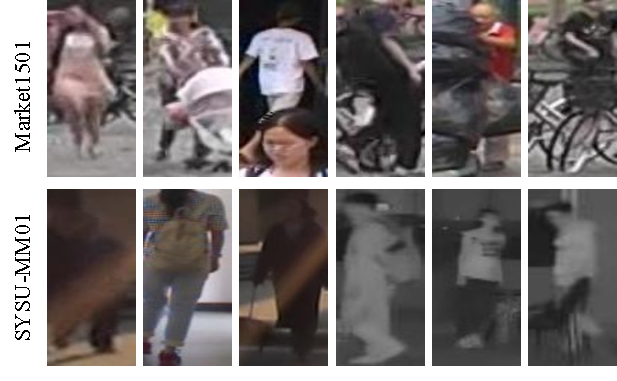
\includegraphics[width=0.8\linewidth]{figs/pdf/outliers.pdf}
\caption{Some outliers detected via the mechanism formulated as Equation.\ref{outliers} on Market1501 and SYSU-MM01 with quartile 0.005.}
\label{fig:outliers}
\end{figure}


\subsubsection{Pose Filtering for 'Failed' Pose Estimation}
\label{PoseValid}
We designed a pose filtering algorithm called PoseValid to eliminate cases where pose extraction has "completely failed." This algorithm checks the validity of the pose keypoints based on factors such as occlusion, keypoint positions, angles, and limb proportions, then get the set of valid poses.
\begin{equation}
S^{\text{trg}}_i = \{ \mathbf{x}_i \mid \text{PoseValid}(\mathbf{x}_i) \text{ and } dis_i \in [Q_p, Q_{1-p}] \}
\end{equation}
where the pose detector in this paper uses pretrained model of DWpose\cite{yang2023effective}. Given a set of keypoints representing a pose, we normalize the pose using the following steps:
\begin{enumerate}
    \item Compute the body height ($h$):\\
    Calculate the Euclidean distance between the Neck (keypoint 1) and the Left Hip (keypoint 11):
    \[
    h = \left\| \mathbf{k}_{\text{Neck}} - \mathbf{k}_{\text{LHip}} \right\|
    \]
    \item Translate the pose:\\
    Shift all keypoints so that the Neck is at the origin:
    \[
    \mathbf{k}'_i = \mathbf{k}_i - \mathbf{k}_{\text{Neck}}
    \]
    \item Scale the pose:\\
    Divide each keypoint by the body height to normalize the size:
    \[
    \mathbf{k}^{\text{normalized}}_i = \frac{\mathbf{k}'_i}{h}
    \]
\end{enumerate}
Then, the filtering process of PoseValid function evaluates the validity of pose keypoints by applying constraints on limb lengths, symmetry, and keypoint positions. 

\subsection{Generation quality and Pose Representation Study}
To assess the quality of the generated images, we replaced the real images in the dataset with images of the same pose and performed inference validation. The results, as shown in Fig.\ref{fig:samepose}, indicate that the original model still successfully matches pedestrians without significant performance degradation. Even with all images in the same pose, the model can effectively differentiate between individuals. This suggests that our generated images are of high quality, retaining the main characteristics of the original images without notably impacting the ReID model. Moreover, we found that pedestrians walking at an angle have higher distinguishability compared to other poses (front, back, and side views), which are more representative of their identities.


\begin{table}[]
\small
\renewcommand{\arraystretch}{1.0}
\renewcommand\tabcolsep{5pt}
\centering
    \begin{tabular}{cc|ccc}
        \hline
        +Ours & +Rerank & mAP & Rank1  \\ \hline
        \ding{55} &\ding{55} & 79.88 & 91.48 \\
        \ding{55} &\ding{51} & 89.56 & 92.07  \\ \hline
        \rowcolor{gray!20}
        \ding{51} &\ding{55} &90.39&94.74\\
        \rowcolor{gray!20}
        \ding{51} &\ding{51}  & \textbf{92.79}&	\textbf{94.83} \\ \hline
    \end{tabular}
    \caption{Compared to k-reciprocal rerank with official settings on Market1501 ($k_1$=20,$k_2$=6).}
    \label{tab:rerank}
\end{table}

\begin{table}[]
\small
\renewcommand{\arraystretch}{1.0}
\renewcommand\tabcolsep{5pt}
\centering
        \begin{tabular}{c|ccc}
        \hline
        Methods & mAP & Rank1  \\ \hline
        TransReID on MSMT17 & 67.80	&85.33\\
        \rowcolor{gray!20}
        +ours & 74.06	&86.55	  \\ \hline
    \end{tabular}
    \caption{Experiment on MSMT17 with TransReID and their official weights.}
    \label{tab:more}
\end{table}


\subsection{More Random Generation}
We provide additional randomly generated images in Fig.\ref{fig:random_all} from Market-1501, SYSU-MM01 and Occluded-ReID datasets.


\subsection{Collaborate with Re-ranking}
Since our method does not change the features' original distribution,
it could collaborate post-processing strategies like rerank, as shown in Tab.\ref{tab:rerank}.

\subsection{Results on MSMT17 with TransReID}
We conduct a simple experiment on MSMT17 dataset with with TransReID and their official pre-trained weights. As shown in Tab.\ref{tab:more}.

\subsection{Comparisons with state-of-the-art methods on three ReID benchmarks}
Comparison on three ReID benchmarks. Since Our method can be applied to any baseline, we choose three methods from three benchmarks which have the official codes and pre-trained weights. With our method, we achieve the new SOTA in three benchmarks, as shown in Fig.\ref{tab:sota_m} and Fig.\ref{tab:sys}.



\begin{table}
\centering
\renewcommand\tabcolsep{5pt}

\begin{tabular}{c|cc|cc}
\hline
 \multirow{2}{*}{Methods}& \multicolumn{2}{c|}{Market1501} & \multicolumn{2}{c}{Occluded-reID} \\ \cline{2-5}
 & Rank-1 & mAP & Rank-1  & mAP \\
\hline
BoT\cite{luo2019bag} & 94.5 & 85.9 & 58.4 & 52.3 \\
PCB\cite{sun2018beyond}& 93.8 & 81.6& - & - \\
VGTri\cite{yang2021learning} & - & - & 81.0 & 71.0 \\
PVPM\cite{gao2020pose} & - & - & 66.8 & 59.5 \\
HOReID\cite{wang2020high} & 94.2 & 84.9 & 80.3 & 70.2 \\
ISP\cite{zhu2020identity} & 95.3 & 88.6 & - & -\\
PAT\cite{li2021diverse} & 95.4 & 88.0 & 81.6 & 72.1 \\
TRANS\cite{he2021transreid} & 95.2 & 88.9 & - & - \\
CLIP\cite{li2023clip} & 95.7 & 89.8 & - & - \\
SOLIDER\cite{chen2023beyond} & 96.9 & 93.9 & - & - \\
SSGR\cite{yan2021occluded} & 96.1 & 89.3 & 78.5 & 72.9 \\
FED\cite{wang2022feature} & 95.0 & 86.3& 86.3 & 79.3 \\
BPBreid\cite{somers2023body} & 95.7 & 89.4 & 82.9 & 75.2\\
PFD\cite{wang2022pose} & 95.5 & 89.7 & 83.0 & 81.5 \\
KPR\textsubscript{IN}\cite{somers2025keypoint} & 95.9 & 89.6 & 85.4 & 79.1 \\
KPR\textsubscript{SOL}\cite{somers2025keypoint} & 96.62 &93.22 &84.83& 82.6\\
\hline
\rowcolor{gray!20}
CLIP+ours & 97.3 & 94.9 & - & -\\
\rowcolor{gray!20}
KPR\textsubscript{IN}+ours & - & - & 91 & 89.34 \\
\hline
\end{tabular}
\caption{Comparisons with state-of-the-art methods on Market1501 and Occluded-reID.}
\label{tab:sota_m}
\end{table}
\begin{table}
\small
\centering
% \renewcommand{\arraystretch}{1.1}
\renewcommand\tabcolsep{5pt}
	\begin{tabular}{l|cc|cc}
		\hline
		\multirow{2}{*}{Methods} & \multicolumn{2}{c|}{All-Search} &\multicolumn{2}{c}{Indoor-Search}\\ \cline{2-5}
              & mAP & Rank-1 & mAP & Rank-1 \\ \cline{1-5}
             PMT\cite{lu2023learning}& 66.13& 67.70& 77.81& 72.95\\
             MCLNet~\cite{hao2021cross}& 61.98 &65.40&76.58 &72.56\\
             MAUM~\cite{Liu2022LearningMU}& 68.79 &71.68& 81.94 &76.9\\
             CAL\cite{CAL}& 71.73 &74.66& 83.68 &79.69\\
             SAAI(w/o AIM)~\cite{fang2023visible}&  71.81& 75.29&  84.6 &81.59\\
             SEFL\cite{feng2023shape}& 72.33 &77.12& 82.95 &82.07\\
             PartMix\cite{kim2023partmix}& 74.62 &77.78& 84.38 &81.52\\
             MID~\cite{Huang2022ModalityAdaptiveMA} & 59.40 &60.27& 70.12 &64.86\\
             FMCNet~\cite{zhang2022fmcnet}& 62.51 &66.34& 74.09 &68.15\\
             MPANet~\cite{wu2021discover}& 68.24 &70.58& 80.95 &76.74\\
             CMT~\cite{jiang2022cross}& 68.57 &71.88& 79.91 &76.90\\
             protoHPE~\cite{zhang2023protohpe}& 70.59 &71.92&81.31 &77.81\\
             MUN~\cite{yu2023modality}& 73.81 &76.24& 82.06 &79.42\\
             MSCLNet~\cite{zhang2022modality}& 71.64 &76.99& 81.17 &78.49\\
             DEEN~\cite{zhang2023diverse}& 71.80 &74.70& 83.30 &80.30\\
             CIFT~\cite{li2022counterfactual}& 74.79 &74.08& 85.61 &81.82\\
             \cline{1-5}
             \rowcolor{gray!20}
            SAAI+ours&76.44&79.33& 86.83& 84.2\\
             \cline{1-5}
	\end{tabular}
             \caption{Comparison with state-of-the-art methods on SYSU-MM01 without re-ranking.}
             \label{tab:sys}                               
\end{table}


% \begin{figure*}
% \centering
% 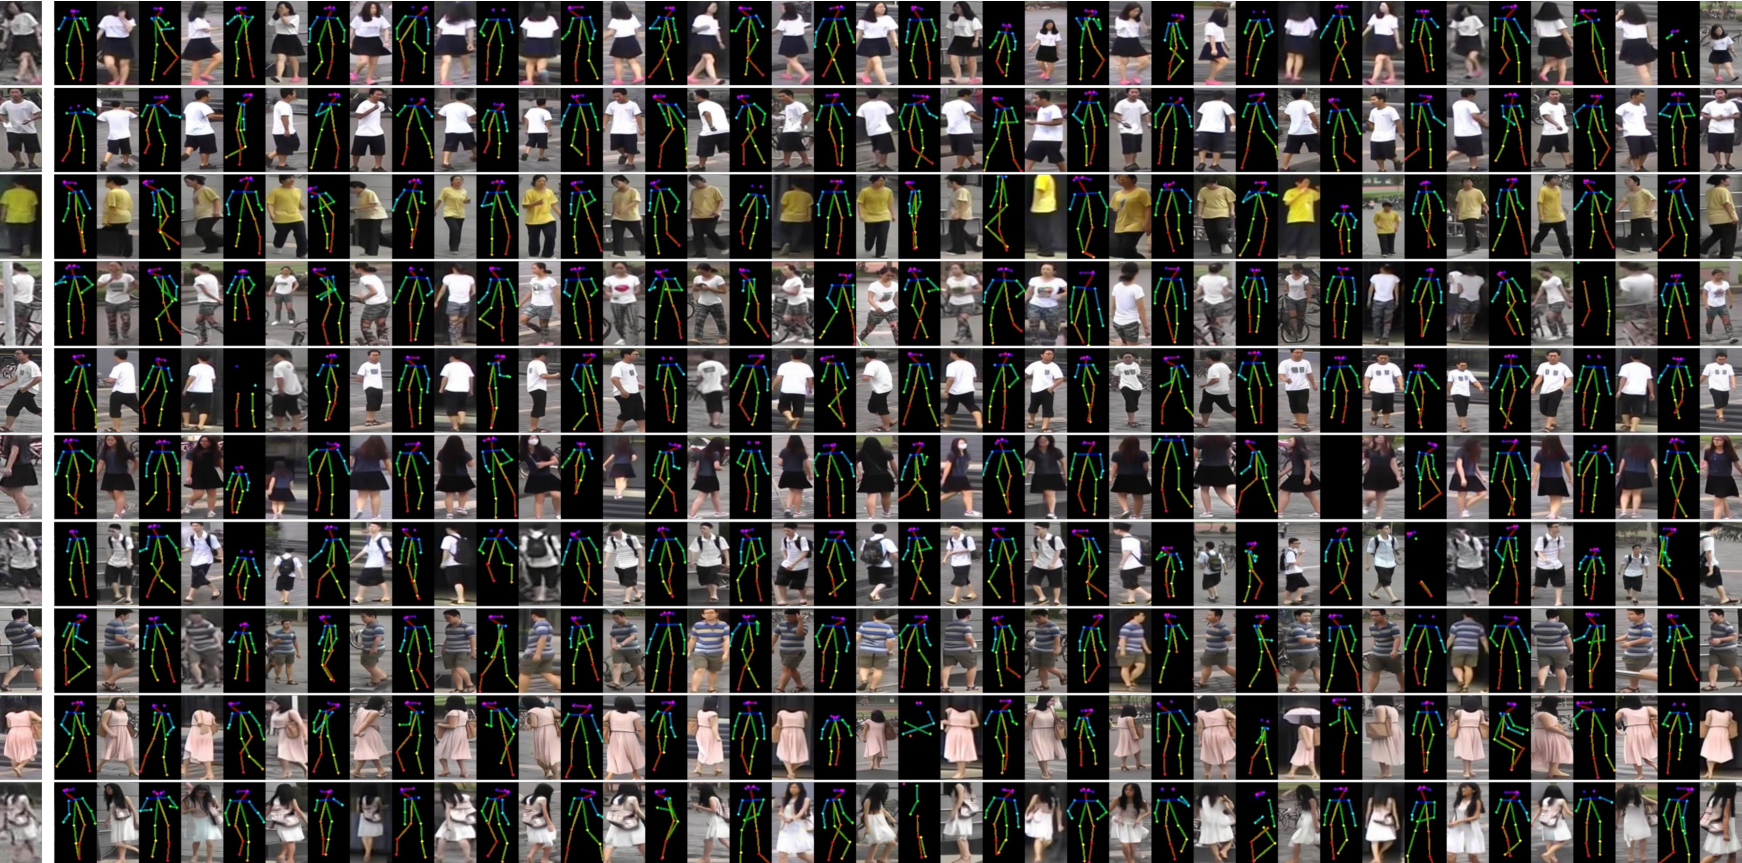
\includegraphics[width=\linewidth]{figs/pdf/random.pdf}
% \caption{Random generated images on Market1501.}
% \label{fig:random_market}
% \end{figure*}

% \begin{figure*}
% \centering
% \includegraphics[width=\linewidth]{figs/pdf/sysu.pdf}
% \caption{Random generated images on SYSU-MM01.}
% \label{fig:random_sysu}
% \end{figure*}


% \begin{figure*}
% \centering
% \includegraphics[width=\linewidth]{figs/pdf/occ.pdf}
% \caption{Random generated images on SYSU-MM01.}
% \label{fig:random_occ}
% \end{figure*}


\subsection{Analysis on quality coefficient $\eta$ of Generation Model}

Fig.\ref{fig:eta} illustrates the effect of adjusting the coefficient $\eta$ on the performance of the ReID model. To evaluate this impact, we gradually increased the value of $\eta$ and observed changes on the mAP and Rank-1 metrics. 

As the value of $\eta$ increases, the performance of the ReID model improves, reaching an optimal point. At $\eta = 2$, both mAP and Rank-1 achieve their maximum values of 88.02\% and 94.77\%, respectively. However, further increasing $\eta$ beyond this point leads to a slight decline in performance. It is easy to find that using generated images to centralize features is effective. However, considering the quality of the generated image, direct adding, although also effective, may not always achieve the best results. Therefore adjusting $\eta$ according to the generation quality of the model in this dataset can better centralize the features.


\subsection{Analysis on $k_1/k_2$ of Neighbor Feature Centralization}
We conducted a detailed analysis of different $k_1$ and $k_2$ combinations, evaluating the results of feature centralization enhancement separately on the Query and Gallery sets, as well as the combined effect (as shown in the Fig.\ref{fig:k1k2}). The selection of these two parameters primarily depends on the number of potential positive samples within the set (adjusting $k_1$) and the confidence in feature associations (adjusting k2). Overall, medium parameter combinations ($k_1$ and $k_2$ in the range of 2-4) provide relatively optimal performance.




























% \begin{equation}
% \mathbf{E}_{i+1} = \text{SiLU}(\text{Conv}_{i, \text{stride}=2}(\text{Conv}_{i}(\mathbf{E}_i)))
% \end{equation}
% \paragraph{Forward Process}

% The Denoising Diffusion Implicit Model (DDIM) \cite{song2020denoising} is fundamental to our approach. The forward process gradually adds Gaussian noise to the data:
% \begin{equation}
% q(\mathbf{z}_t \mid \mathbf{z}_{t-1}) = \mathcal{N}(\mathbf{z}_t; \sqrt{\alpha_t} \mathbf{z}_{t-1}, (1 - \alpha_t) \mathbf{I})
% \end{equation}
% where \( \alpha_t \) controls the noise schedule, and \( \mathbf{z}_t \) is the noisy latent at timestep \( t \).

% \paragraph{Reverse Process}

% The model learns to reverse the diffusion process with classifier-free guidance \cite{ho2022classifier}:
% \begin{equation}
% \begin{aligned}
%     \mathbf{z}_{t-1} &= \boldsymbol{\mu}(\mathbf{z}_t, t, \mathbf{E}_{\text{pose}}, \mathbf{H}) - w \cdot (\hat{\boldsymbol{\epsilon}}^{\text{cond}} - \hat{\boldsymbol{\epsilon}}^{\text{uncond}}) \\
%     \hat{\boldsymbol{\epsilon}}^{\text{cond}} &= \boldsymbol{\epsilon}_{\theta}(\mathbf{z}_t, t, \mathbf{E}_{\text{pose}}, \mathbf{H}) \\
%     \hat{\boldsymbol{\epsilon}}^{\text{uncond}} &= \boldsymbol{\epsilon}_{\theta}(\mathbf{z}_t, t, \mathbf{E}_{\text{pose}}, \mathbf{H} = 0)
% \end{aligned}
% \end{equation}

% The model predicts the mean \( \boldsymbol{\mu} \) of the posterior distribution at each timestep, conditioned on the pose features and conditioning embedding.
% \begin{equation}
% \small
% \boldsymbol{\mu}(\mathbf{z}_t, t, \mathbf{E}_{\text{pose}}, \mathbf{H}) = \frac{1}{\sqrt{\alpha_t}} \left( \mathbf{z}_t - \frac{1 - \alpha_t}{\sqrt{1 - \bar{\alpha}_t}} \boldsymbol{\epsilon}_{\theta}(\mathbf{z}_t, t, \mathbf{E}_{\text{pose}}, \mathbf{H}) \right)
% \end{equation}
% \( \hat{\boldsymbol{\epsilon}} \) is the predicted noise by the denoising UNet, and \( \bar{\alpha}_t = \prod_{s=1}^{t} \alpha_s \).